\chapter{El método científco}

\begin{cita}{Galileo Galilei.}El Universo está escrito en el lenguaje de las matemáticas y sus caracteres son triángulos, círculos y otras figuras geométricas, sin las cuales es humanamente imposible entender una sola de sus palabras. Sin ese lenguaje, navegamos en un oscuro laberinto.
\end{cita}

\section{¿Qué es la física?}
 
La física (del latín \textit{physica}, y este del griego antiguo \textit{$\phi$$\upsilon$$\sigma$$\iota$$\kappa$o$\varsigma$}, «natural, relativo a la naturaleza») es la ciencia natural que estudia los componentes fundamentales del Universo, la energía, la materia, el espacio-tiempo y las interacciones fundamentales. La física es una ciencia básica estrechamente vinculada con las matemáticas y la lógica en la formulación y cuantificación de sus principios. 

El alcance de la física es extraordinariamente amplio y puede incluir estudios tan diversos como la mecánica cuántica, la física teórica o la óptica. La física moderna se orienta a una especialización creciente, donde los investigadores tienden a enfocar áreas particulares más que a ser universalistas, como lo fueron Albert Einstein o Lev Landau, que trabajaron en una multiplicidad de áreas.

La física es tal vez la más antigua de todas las disciplinas académicas, ya que la astronomía es una de sus subdisciplinas. También comenzó hace más de dos mil años con los primeros trabajos de filósofos griegos. En los últimos dos milenios, la física fue considerada parte de lo que ahora llamamos filosofía, química y ciertas ramas de la matemática y la biología, pero durante la Revolución Científica en el siglo XVII se convirtió en una ciencia moderna, única por derecho propio. Sin embargo, en algunas esferas como la física matemática, la química cuántica y la biofísica (por ejemplo) los límites de la física con otras ramas de la ciencia siguen siendo difíciles de distinguir. La formulación de las teorías sobre las leyes que gobiernan el Universo ha sido un objetivo central de la física desde tiempos remotos, con la filosofía del empleo sistemático de experimentos cuantitativos de observación y prueba como fuente de verificación. La clave del desarrollo histórico de la física incluye hitos como la ley de la gravitación universal y la mecánica clásica de Newton, la comprensión de la naturaleza de la electricidad y su relación con el magnetismo de Faraday, la teoría de la relatividad especial y teoría de la relatividad general de Einstein, el desarrollo de la termodinámica con James Prescott Joule y Sadi Carnot y el modelo de la mecánica cuántica a los niveles de la física atómica y subatómica con Louis-Victor de Broglie, Heisenberg y Erwin Schrödinger. 

Esta disciplina incentiva competencias, métodos y una cultura científica que permiten comprender nuestro mundo físico y viviente, para luego actuar sobre él. Sus procesos cognitivos se han convertido en protagonistas del saber y hacer científico y tecnológico general, ayudando a conocer, teorizar, experimentar y evaluar actos dentro de diversos sistemas, clarificando causa y efecto en numerosos fenómenos. De esta manera, la física contribuye a la conservación y preservación de recursos, facilitando la toma de conciencia y la participación efectiva y sostenida de la sociedad en la resolución de sus propios problemas.

La física es significativa e influyente, no solo debido a que los avances en la comprensión a menudo se han traducido en nuevas tecnologías, sino también a que las nuevas ideas en la física resuenan con las demás ciencias, las matemáticas y la filosofía.

La física no es sólo una ciencia teórica; es también una ciencia experimental. Como toda ciencia, busca que sus conclusiones puedan ser verificables mediante experimentos y que la teoría pueda realizar predicciones de experimentos futuros basados en observaciones previas. Dada la amplitud del campo de estudio de la física, así como su desarrollo histórico con relación a otras ciencias, se la puede considerar la ciencia fundamental o central, ya que incluye dentro de su campo de estudio a la química, la biología y la electrónica, además de explicar sus fenómenos. 

La física, en su intento de describir los fenómenos naturales con exactitud y veracidad, ha llegado a límites impensables: el conocimiento actual abarca desde la descripción de partículas fundamentales microscópicas hasta el nacimiento de las estrellas en el universo e incluso el poder conocer con una gran probabilidad lo que aconteció en los primeros instantes del nacimiento de nuestro universo, por citar unos pocos campos.

\subsection{Un poco de historia}

\begin{small}
La historia de la física abarca los esfuerzos y estudios realizados por las personas que han tratado de entender el porqué de la naturaleza y los fenómenos que en ella se observan: el paso de las estaciones, el movimiento de los cuerpos y de los astros, los fenómenos climáticos, las propiedades de los materiales, entre otros. Gracias a su vasto alcance y a su extensa historia, la física es clasificada como una ciencia fundamental. Esta disciplina científica se puede dedicar a describir las partículas más pequeñas o a explicar cómo nace una estrella.
 
La mayoría de las civilizaciones de la antigüedad trataron desde un principio de explicar el funcionamiento de su entorno; miraban las estrellas y pensaban cómo ellas podían regir su mundo. Esto llevó a muchas interpretaciones de
carácter más filosófico que físico; no en vano en esos momentos a la física se le llamaba filosofía natural. Muchos
filósofos se encuentran en el desarrollo primitivo de la física, como Aristóteles, Tales de Mileto o Demócrito, ya que fueronlosprimerosentratardebuscaralgúntipodeexplicaciónalosfenómenosquelesrodeaban. Las primeras explicaciones que aparecieron en la antigüedad se basaban en consideraciones puramente filosóficas, sin verificarse experimentalmente. Algunas interpretaciones equivocadas, como la hecha por Claudio Ptolomeo en su famoso Almagesto —«La Tierra está en el centro del Universo y alrededor de ella giran los astros»— perduraron durante miles de años. A pesar de que las teorías descriptivas del universo que dejaron estos pensadores eran erradas en sus conclusiones, estas tuvieron validez por mucho tiempo, casi dos mil años, en parte por la aceptación de la Iglesia católica de varios de sus preceptos, como la teoría geocéntrica. 
 
Esta etapa, denominada oscurantismo en la ciencia de Europa, termina cuando el canónigo y científico Nicolás Copérnico, quien es considerado padre de la astronomía moderna, recibe en 1543 la primera copia de su libro, titulado De Revolutionibus Orbium Coelestium. A pesar de que Copérnico fue el primero en formular teorías plausibles, es otro personaje al cual se le considera el padre de la física como la conocemos ahora. Un catedrático de matemáticas de la Universidad de Pisa a finales del siglo XVI cambiaría la historia de la ciencia, empleando por primera vez experimentos para comprobar sus afirmaciones: Galileo Galilei. Mediante el uso del telescopio para observar el firmamento y sus trabajos en planos inclinados, Galileo empleó por primera vez el método científico y llegó a conclusiones capaces de ser verificadas. A sus trabajos se les unieron grandes contribuciones por parte de otros científicos como Johannes Kepler, Blaise Pascal y Christian Huygens.

Posteriormente, en el siglo XVII, un científico inglés reunió las ideas de Galileo y Kepler en un solo trabajo, unifica las ideas del movimiento celeste y las de los movimientos en la Tierra en lo que él llamó gravedad. En 1687, Isaac Newton formuló, en su obra titulada Philosophiae Naturalis Principia Mathematica, los tres principios del movimiento y una cuarta ley de la gravitación universal, que transformaron por completo el mundo físico; todos los fenómenos podían ser vistos de una manera mecánica. 

El trabajo de Newton en este campo perdura hasta la actualidad, ya que todos los fenómenos macroscópicos pueden ser descritos de acuerdo a sus tres leyes. Por eso durante el resto de ese siglo y en el posterior, el siglo XVIII, todas las investigaciones se basaron en sus ideas. De ahí que se desarrollaron otras disciplinas como la termodinámica, la óptica, la mecánica de fluidos y la mecánica estadística. Los conocidos trabajos de Daniel Bernoulli, Robert Boyle y Robert Hooke, entre otros, pertenecen a esta época. 

En el siglo XIX se produjeron avances fundamentales en la electricidad y el magnetismo, principalmente de la mano de Charles-Augustin de Coulomb, Luigi Galvani, Michael Faraday y Georg Simon Ohm, que culminaron en el trabajo de James Clerk Maxwell en 1855, que logró la unificación de ambas ramas en el llamado electromagnetismo. Además, se producen los primeros descubrimientos sobre radiactividad y el descubrimiento del electrón por parte de Joseph John Thomson en 1897.

Durante el sigloXX, la física se desarrolló plenamente. En1904, Hantaro Nagaoka había propuesto el primer modelo del átomo, el cual fue confirmado en parte por Ernest Rutherford en 1911, aunque ambos planteamientos serían después sustituidos por el modelo atómico de Bohr, de 1913. En 1905, Einstein formuló la teoría de la relatividad especial, la cual coincide con las leyes de Newton al decir que los fenómenos se desarrollan a velocidades pequeñas comparadas con la velocidad de la luz. En 1915 extendió la teoría de la relatividad especial, formulando la teoría de la relatividad general, la cual sustituye a la ley de gravitación de Newton y la comprende en los casos de masas pequeñas. Max Planck, Albert Einstein, Niels Bohr y otros, desarrollaron la teoría cuántica, a fin de explicar resultados experimentales anómalos sobre la radiación de los cuerpos. En 1911, Ernest Rutherford dedujo la existencia de un núcleo atómico cargado positivamente, a partir de experiencias de dispersión de partículas. En 1925 Werner Heisenberg, y en 1926 Erwin Schrödinger y Paul Adrien Maurice Dirac, formularon la mecánica cuántica, la cual comprende las teorías cuánticas precedentes y suministra las herramientas teóricas para la Física de la materia condensada. 

Posteriormente se formuló la teoría cuántica de campos, para extender la mecánica cuántica de acuerdo con la Teoría de la Relatividad especial, alcanzando su forma moderna a finales de la década de 1940, gracias al trabajo de Richard Feynman, Julian Schwinger, Shin'ichiro Tomonaga y Freeman Dyson, los cuales formularon la teoría de la electrodinámica cuántica. Esta teoría formó la base para el desarrollo de la física de partículas. En 1954, Chen Ning Yang y Robert Mills desarrollaron las bases del modelo estándar. Este modelo se completó en los años 1970, y con él fue posible predecir las propiedades de partículas no observadas previamente, pero que fueron descubiertas sucesivamente, siendo la última de ellas el quark top.

Los intentos de unificar las cuatro interacciones fundamentales han llevado a los físicos a nuevos campos impensables. Las dos teorías más aceptadas, la mecánica cuántica y la relatividad general, que son capaces de describir con gran exactitud el macro y el micromundo, parecen incompatibles cuando se las quiere ver desde un mismo punto de vista. Por eso se han formulado nuevas teorías, como la supergravedad o la teoría de cuerdas, donde se centran las investigaciones a inicios del siglo XXI. Esta ciencia no desarrolla únicamente teorías, también es una disciplina de experimentación. Sus hallazgos, por lo tanto, pueden ser comprobados a través de experimentos. Además, sus teorías permiten establecer previsiones sobre pruebas que se desarrollen en el futuro.
\end{small}

\begin{figure}[H]
	\centering
	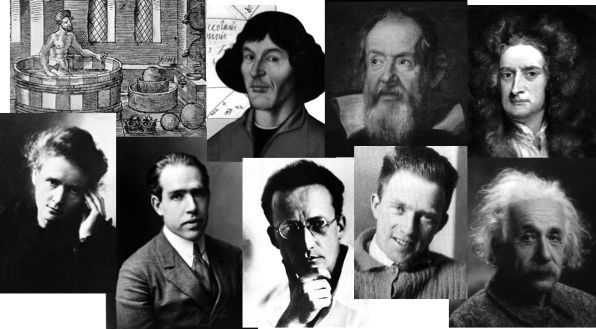
\includegraphics[width=1\textwidth]{imagenes/imagenes01/T01IM01.png}
	\caption{Arquímedes, Copérnico, Galileo, Newton, Marie Curie, Bohr, Schrödinger, Heisenberg y Einstein. \scriptsize{(Imagen del prof. Augusto Beléndez Vázquez, Universidad de Alicante.)}}
	\end{figure}

\subsection{Ramas de la física} 
\begin{itemize}
	\item Mecánica Clásica 
	\item Mecánica cuántica
	\item Teoría cuántica de campos 
	\item Teoría de la relatividad 
	\begin{itemize}
	\item Relatividad especial  
	\item Relatividad general 
     \end{itemize}
\item Mecánica Estadística 
\item Termodinámica
\item Mecánica de medios continuos 
\begin{itemize}
	\item Mecánica del sólido rígido, Mecánica de sólidos deformables, Elasticidad, Plasticidad.
	\item Mecánica de fluidos. 
\end{itemize}
Electromagnetismo 
\begin{itemize}
	\item Electricidad 
	\item Magnetismo 
\end{itemize}
\item Electrónica 
\item Astrofísica 
	\begin{itemize} \item Cosmología \end{itemize}
\item Geofísica (rama de la geología) 
\item Biofísica (rama de la biología) 
\item Óptica \footnote{Fuente: Wikipedia}
\end{itemize}


\subsection{La física según los físicos}


\begin{changemargin}{1cm}{1cm}

\textit{``La física es una ciencia cuyo objetivo es estudiar los componentes de la materia y sus interacciones mutuas. En función de estas interacciones la Física explica las propiedades de la materia en conjunto, así como los distintos fenómenos que observamos en la Naturaleza''.}  \small{(M. Alonso y E. J. Finn, ``Física. Vol. I: Mecánica'', Addison-Wesley Iberoamericana. México, 1986)}\normalsize{.} 


\vspace{2mm} \textit{``La historia de la física no puede entenderse como una mera yuxtaposición de descubrimientos y de observaciones experimentales a la cual se agregue su descripción matemática para dar lugar a teorías, sino que es también historia de los conceptos''}. \small{(Werner Heisenberg)}\normalsize{.} 


\textit{``La física se propone descubrir y dar forma matemática a las leyes universales que relacionan entre sí las magnitudes que intervienen en los fenómenos reales''.} \small{(Julio Palacios)}\normalsize{.} 

\textit{``La física es una creación del intelecto humano en su intento por comprender el mundo físico''. ``No es una mera colección de leyes, un catálogo de hechos sin relación mutua, sino que es una creación de la mente humana, con sus ideas y conceptos libremente inventados. Las teorías físicas tratan de dar una imagen de la realidad y de establecer su conexión con el amplio mundo de las impresiones sensoriales. La única justificación de nuestras estructuras mentales es si esa conexión se logra y de qué modo se hace'' }. \small{(Albert Einstein)}\normalsize{.} 

\textit{``Es equivocado pensar que la tarea de la física es averiguar cómo es la naturaleza. La física se refiere a lo que nosotros podemos decir de ella''}. (\small{Niels Bohr)}\normalsize{.} 

\textit{``La física es la ciencia de lo exótico, pero también es la ciencia de la vida cotidiana.''}  \small{(P. A. Tipler, ``Física para la ciencia y la tecnología'', Vol. 1 -Ed. Reverté. Barcelona, 1999)}\normalsize{.} 

\textit{``El cosmos también está dentro de nosotros: estamos hechos de materia estelar, y somos el medio para que el cosmos se conozca a sí mismo''.}\small{(Carl Sagan)}\normalsize{.}

\textit{``El milagro de la adecuación del lenguaje de las matemáticas para la formulación de las leyes físicas es un regalo maravilloso que ni entendemos ni merecemos''.}\small{(Eugene Wigner)}\normalsize{.}

\textit{``La ciencia es física. Todo lo demás es filatelia''.}\small{(Ernest Rutherford)}\normalsize{.}

\textit{``La ciencia será siempre una búsqueda, jamás un descubrimiento real. Es un viaje, nunca una llegada''.}\small{(Karl Popper)}\normalsize{.}

\textbf{\textit{``La física es lo ocupa a los físicos hasta avanzadas horas de la madrugada''.}} \small{(Richard Feynman)}\normalsize{.} Tal vez, la mejor definición de física.

\end{changemargin}

\textit{``La Física es como el sexo''}, dijo en cierta ocasión Richard Feynman.  \textit{``Está claro que puede tener algunos resultados prácticos, pero no lo hacemos por eso.''} La célebre cita de Feynman es perfectamente aplicable a toda la investigación científica básica.	
	

En conclusión, la física es mejor definirla en función de lo que se ocupa. Así, física es la ciencia que se ocupa de estudiar la mecánica clásica, la teoría cinética de gases, la teoría de campos, $\cdots$

\section{Conocimiento científico vs conocimiento ordinario}


Es \emph{conocimiento científico} es el que  adquiere el ser humano mediante los instrumentos de la metodología científica. El \emph{conocimiento ordinario} es el que adquiere por la experiencia y el sentido común.

Entre ambos tipos de conocimiento hay una estrecha relación: \emph{lo que hoy es conocimiento científico, mañana puede ser conocimiento ordinario}. Un claro ejemplo lo tenemos en la visión heliocentrista frente a la geocentrista, lo que hoy es conocimiento ordinario --la tierra gira entorno al sol-- hace unos siglos era considerado conocimiento científico.

\vspace{2mm}\centerline{\colorbox{LightYellow}{Experiencia + sentido común $\to$ conocimiento ordinario.}}\justify

 El objetivo de ambos tipos de conocimiento es objetivizar el mundo y racionalizarlo. 

\colorbox{LightYellow}{Conocimiento científico:} empieza donde acaba el conocimiento ordinario y para adquirirlo se precisa hacer uso del \colorbox{LightYellow}{\textit{`método científico'.}}

\section{El método científico}

Un `sistema científico' es una porción de universo que va a ser objeto de nuestro estudio.

El método científico es la sistemática formal de investigación que permite al físico interpretar los distintos problemas o fenómenos que se dan en ese sistema científico.

Pero ese método no es algo rígido, no hay un sistema fijo de reglas que nos permitan interpretar de una manera unívoca los fenómenos de ese sistema científico. El método científico no es un sistema inmutable. Ahora es válido, pues no contamos con otro, pero pueden inventarse otras leyes que se puedan aplicar a ese sistema científico.

El método científico se basa en:

\vspace{-2mm}\begin{itemize}
\item Tenemos un determinado sistema científico.
\vspace{-2mm} \item En él se dan una serie de fenómenos.
\vspace{-2mm} \item Nuestro objeto será interpretar esos fenómenos.	
\end{itemize}


\emph{Pasos a seguir para estudiar los fenómenos de cualquier sistema científico:}

\begin{enumerate}[a) ]
	\vspace{-2mm}\item Se formula el fenómeno $A$ \emph{con precisión y específicamente}.
	\vspace{-2mm}\item Observación de los \emph{hechos significativos} del fenómeno (los que nos ayuda a afirmar o refutar una ley).
	\vspace{-2mm}\item Proposición de \emph{hipótesis}, para explicar esos hechos significativos.
	\vspace{-2mm}\item Si las proposiciones formuladas en b) son correctas ascienden a la categoría de \emph{ley particular científica} (particular al fenómeno $A$).
	
	Si es correcta esta ley científica, nos explicará los hechos significativos y nos esclarecerá otros que aún no habíamos observado.
\end{enumerate}


Luego se repite esta operación con los fenómenos $B$, $C$, etc.

Finalmente, por \emph{inducción} de los fenómenos $A$, $B$, $C$, $\cdots$, es posible que se obtenga una \emph{ley general}. Si es válida, podremos llegar a descubrir nuevos fenómenos en nuestro sistema físico.

La ciencia que más se aproxima a este método es la \emph{física}.

\begin{ejem}{Galileo. Fenómeno $A$: `Caída libre de graves'}

Hechos significativos:
\vspace{-2mm}\begin{itemize}
	\item Observa que no influye la masa.
	\vspace{-2mm}\item Observa que \emph{casi} no influye el rozamiento con el aire.
	\vspace{-2mm}\item Observa que sí influye el tiempo: hay variación de la velocidad. Empieza a a caer lentamente y la velocidad va aumentando con el tiempo (aceleración).
\end{itemize}

Hipótesis: La aceleración es constante (de aquí se deduce una ley científica).
\end{ejem}

\begin{ejem}{Keppler. Fenómeno B: ¿De qué forma orbitan los planetas al sol?}

Hechos significativos:
\begin{itemize}
\vspace{-2mm} \item $2^a$ ley de Keppler: ``Las áreas barridas por unidad de tiempo es una constante'' (la velocidad areolar -- de áreas -- es constante).	
\end{itemize}

Hipótesis: Las órbitas son elípticas (esta hipótesis está de acuerdo con los hechos significativos).

De aquí se deducen sus tres leyes:
\vspace{-2mm}\begin{itemize} 
\vspace{-2mm}\item [-] Vueltas elípticas.
\vspace{-2mm}\item [-] Velocidad areolar constante.
\vspace{-2mm}\item [-] Los cuadrados de los tiempos de revolución coinciden con los cubos de los semi-ejes mayores de las elipses.
\end{itemize}	
\end{ejem}

\begin{ejem}{Newton: Ley de Gravitación Universal}

Intuye la ley de inercia a partir de la ley de caída de graves.

Con sus leyes construye el edificio de la mecánica clásica.	

Aplica a las observaciones de Keppler la mecánica y así obtiene la ``ley de gravitación universal''. Se trata de una `ley general', obtenida por inducción de las leyes de Galileo (Fenómeno $A$) y Keppler (fenómeno $B$). Explica estas leyes y las critica, ve sus fallos:

\begin{itemize}
\item [---] A Galileo: la aceleración no es constante, solo es aproximadamente constante.
\item [---] A Keppler: 
	\begin{itemize}
	\item [-] La órbitas no son totalmente elípticas. 	
	\item [-] La velocidad areolar es aproximadamente constante.
	\item [-] Los tiempos de revolución al cuadrado son aproximadamente igual a los cubos de los semiejes mayores.
	\end{itemize}
\end{itemize}
\end{ejem}

\begin{multicols}{2}
Más tarde se observa que Mercurio no describe una elipse, su eje se desvía, describe una `roseta'.

La segunda ley de Newton ya no es válida.

Aparece una ley mejor que la anterior: ``Teoría de la Relatividad General'', de Albert Einstein.
\begin{figure}[H]
	\centering
	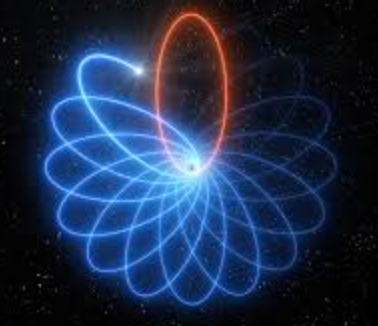
\includegraphics[width=.4\textwidth]{imagenes/imagenes01/T01IM02.png}
	\end{figure}
\end{multicols}

\begin{multicols}{2}
$\quad$

Los rayos de luz se comportan como si tuviesen `masa': cuando un rayo de luz pasa por el lado de un cuerpo pesado siente la acción de la gravedad de éste y el haz se curva.

\begin{figure}[H]
	\centering
	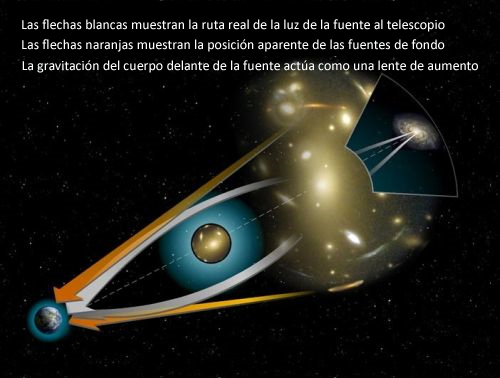
\includegraphics[width=.4\textwidth]{imagenes/imagenes01/T01IM03.png}
	\end{figure}
\end{multicols}	
	

\section{Modelo matemático de un sistema físico}
	
En un sistema físico, por ejemplo el conjunto `Tierra-Sol' hay multitud de fenómenos que observar. Centrémonos en el estudio del periodo de revolución de la Tierra alrededor del Sol. Ahora es cuando aparece el \emph{modelo matemático} del sistema físico.

\begin{figure}[H]
	\centering
	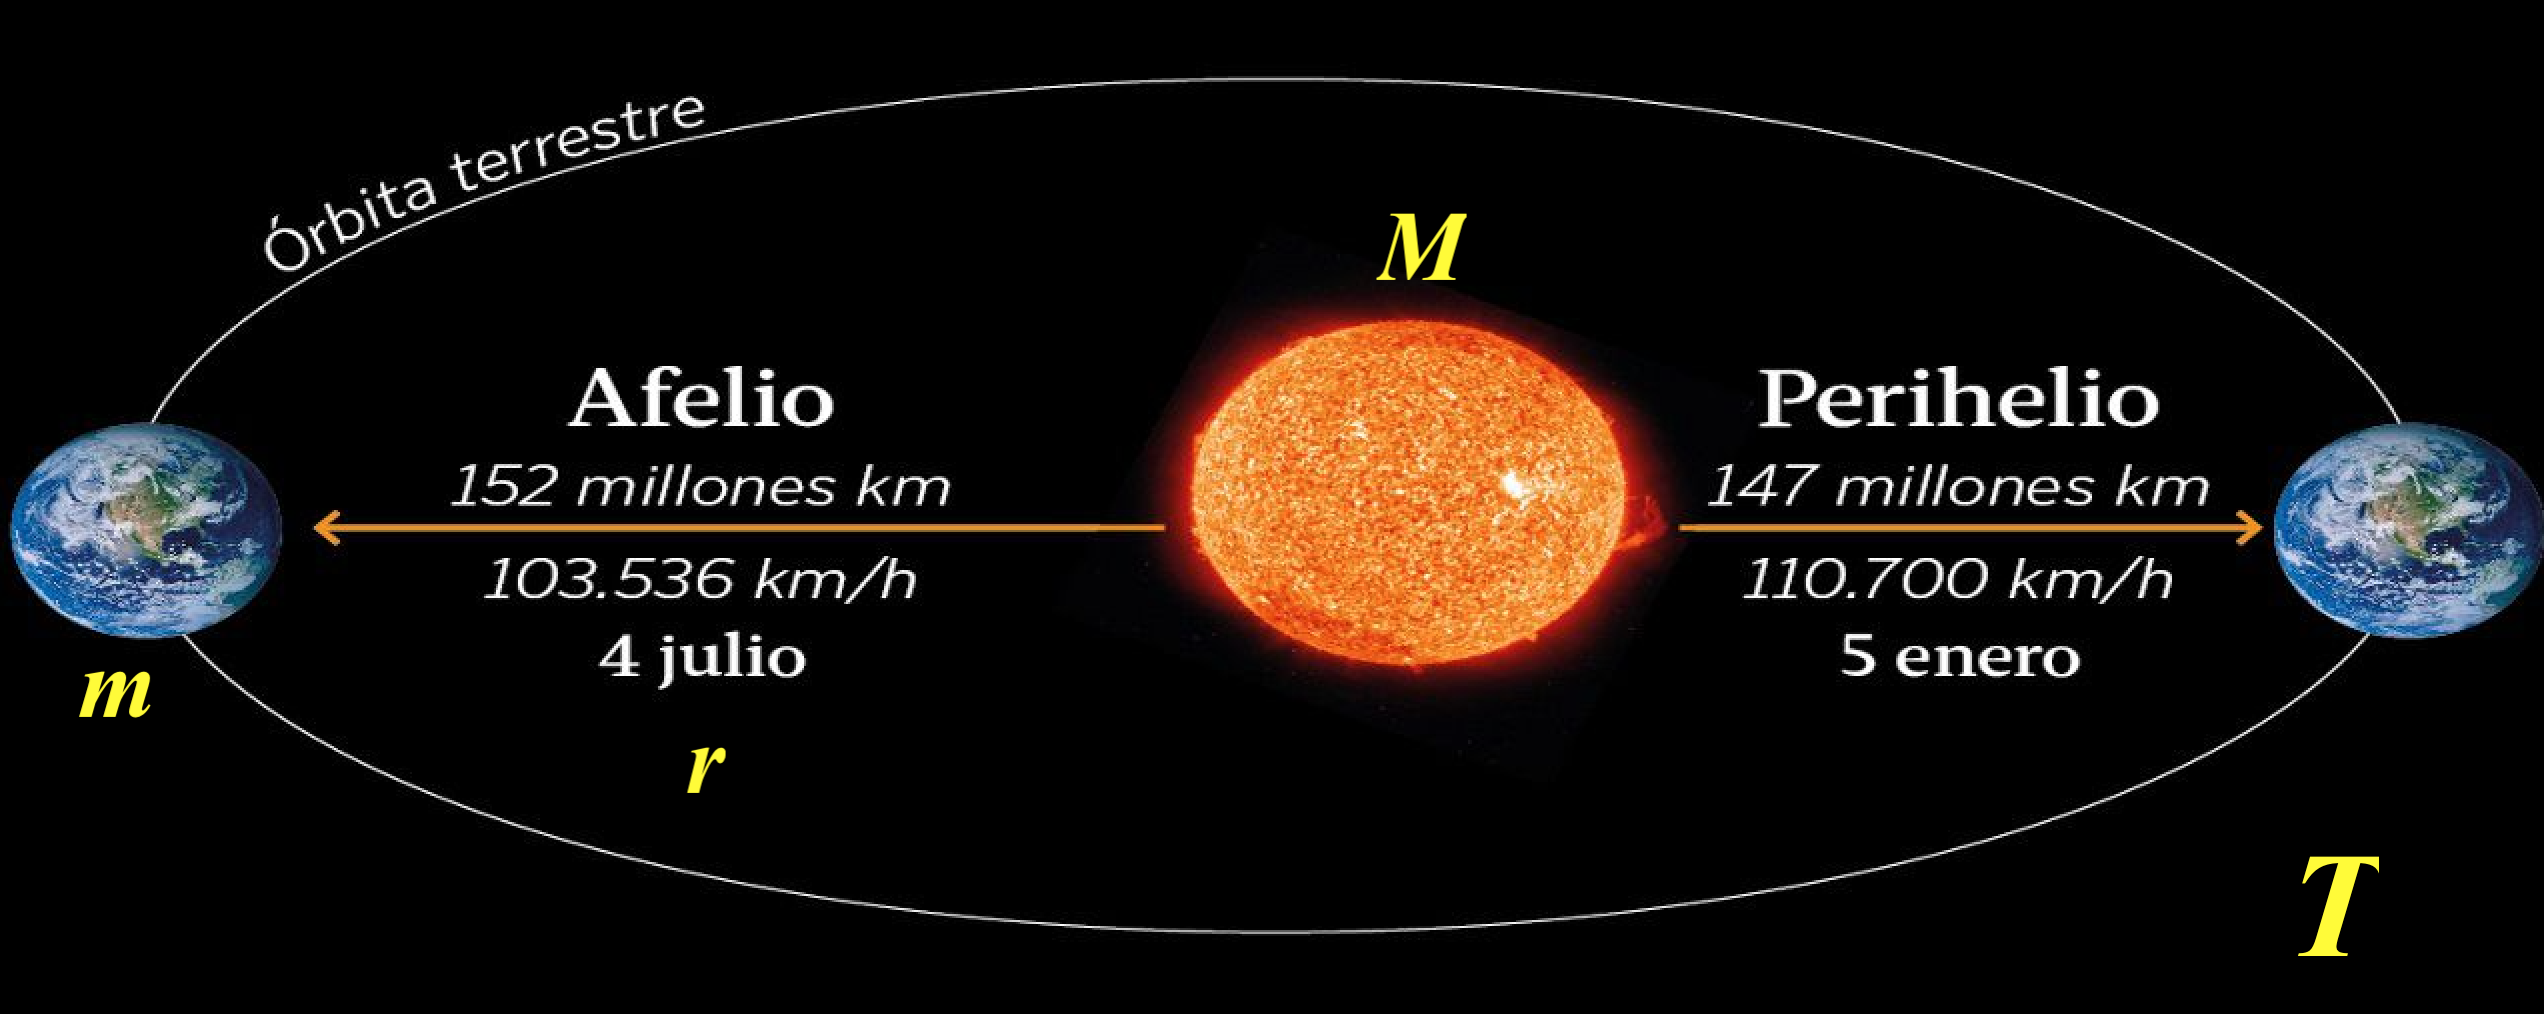
\includegraphics[width=.9\textwidth]{imagenes/imagenes01/T01IM04.png}
	\end{figure}
	
Aplicando las leyes de la mecánica a este modelo matemático encontraremos el periodo de revolución, $T$. Si el modelo es bueno, está de acuerdo con la experiencia, usaremos esta fórmula para, por ejemplo, la rotación del electrón alrededor del núcleo de Hidrógeno.

\vspace{10mm} %****************************
¿Cuántos modelos matemáticos puede tener un sistema físico? Respuesta: ``Un sistema físico puede tener tantos modelos matemáticos como fenómenos haya que estudiar en él''.
	
\newpage %**********************************************
\begin{myblock}{Feynman y la física.}
\begin{small}	
Entre 1961 y 1963, el famoso científico Richard Feynman dio una serie de conferencias de física en Caltech. Las notas de esas clases fueron luego compiladas y presentadas como \textbf{The Feynman Lectures}, y son considerados los libros de física más exitosos de la historia, con más de 1.5 millones de copias vendidas. 
 
\vspace{2mm} ``Uno podría preguntar, porqué es que no podemos enseñar física mostrando primero las leyes básicas y luego demostrando cómo funcionan en todas las circunstancias posibles, de la misma forma en que lo hacemos con la geometría euclidiana, donde enunciamos los axiomas y luego hacemos todo tipo de deducciones. No lo podemos hacer de esta manera por dos razones: en primera, porque aún no conocemos todas las leyes básicas, de hecho existe una ‘frontera creciente’ de ignorancia. Y en segunda, la correcta enunciación de las leyes físicas involucra ideas poco familiares que requieren de matemáticas avanzadas para su descripción. Por lo tanto, requerimos de una cantidad considerable de preparación tan sólo para saber lo que significan las palabras que estamos usando en estas leyes. Siendo así, no podemos enunciarlas en general, sino sólo de parte en parte.
Ahora bien, cada parte del total de la naturaleza es una aproximación a la verdad completa, o bien la verdad completa tal y como la podemos concebir. De hecho, todo lo que sabemos no es más que un tipo de aproximación, porque sabemos que no conocemos todas las leyes. Por lo tanto, las cosas que aprendemos deben ser desaprendidas más tarde, o por lo menos corregidas.''

\vspace{2mm} ``El principio de la ciencia, o más bien casi su definición, es ésta: La prueba de todo conocimiento es el experimento. El experimento es el único juez de una verdad científica.''

\vspace{2mm} ``Finalmente, y lo más interesante, es que filosóficamente estamos diciendo que esta ley de aproximación hace que siempre estemos equivocados: aún un efecto muy pequeño en nuestro conocimiento puede tener implicaciones muy profundas en nuestras ideas acerca del mundo.''
\end{small}
\hspace{20mm} \rightline{\textit{\normalsize{Por Alfonso Araujo, el 6 agosto, 2019. }}NAUKAS.}
\end{myblock}

